% !TeX root = main.tex

\section{Architecture du projet}
\label{sec:architecture}

L'outil a été écrit en Python (version 3.10), un langage qui dispose de nombreuses bibliothèques pour traiter les images, suivant l'état de l'art. Plutôt qu'un programme en un seul bloc, le choix s'est porté sur une série de scripts capables de s'adapter aux particularités de chaque registre de chaque géomètre. 


Pour l'un des registres du cabinet, un classeur Excel existait déjà avec une partie des informations. Un script Python a été écrit pour lire ce classeur et lier directement les pages scannées aux données de ce fichier. Cela évite la saisie manuelle des informations déjà connues.

La Figure~\ref{fig:architecture_pfe} montre l'organisation générale de l'outil. Le programme principal (\texttt{main}) s'occupe de lancer les différents scripts dans l'ordre :
\begin{itemize}
  \item Le tri du document (\texttt{plan\_classifieur.py}).
  \item Le repérage et le découpage des zones utiles par YOLOv8 (\texttt{spatial\_extracteur.py}).
  \item La lecture du texte et l'extraction des mots-clés (\texttt{outil\_ocr.py}).
  \item La vérification de la cohérence des données (\texttt{coherence\_controle.py}).
  \item L'interface de relecture et de correction sous Streamlit (\texttt{app\_validation.py}).
  \item L'envoi des données vers Géofoncier (\texttt{geofoncier\_api.py}).
\end{itemize}

\begin{figure}[H]
  \centering
  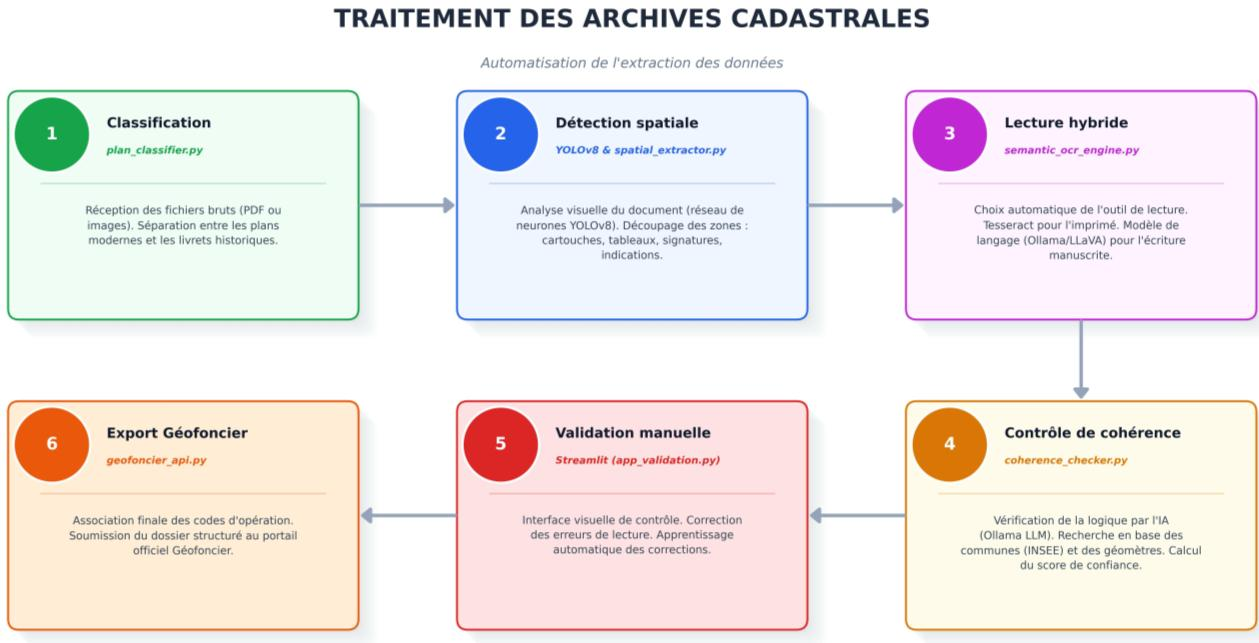
\includegraphics[width=\textwidth]{img/r4p_page2_img1.jpeg}
  \caption{Organigramme des solutions retenues et enchaînement des scripts Python.}
  \label{fig:architecture_pfe}
\end{figure}

Cette séparation en différents scripts permet de dérouler le traitement étape par étape et de modifier plus facilement le code, mais également d'adapter le traitement à de nouveaux cas. La sous-section suivante détaille les outils utilisés et la structure du projet.

\subsection{Environnement technique et organisation du code}

Tout l'outil fonctionne directement sur l'ordinateur du cabinet sous Windows. Aucune donnée n'est envoyée sur Internet, ce qui garantit le respect du secret professionnel évoqué plus tôt.

Les outils et bibliothèques utilisés dans le projet sont les suivants :
\begin{itemize}
  \item PyMuPDF (fitz) : lecture des fichiers PDF créés sur ordinateur (\href{https://github.com/pymupdf/PyMuPDF}{Dépôt PyMuPDF}).
  \item OpenCV et NumPy : nettoyage des images, redressement des lignes et réglage du contraste (\href{https://github.com/opencv/opencv}{Dépôt OpenCV}).
  \item Ultralytics YOLOv8 : repérage et découpage des zones utiles sur la page (\href{https://github.com/ultralytics/ultralytics}{Dépôt YOLOv8}).
  \item PyLaia : lecture de l'écriture manuscrite (\href{https://github.com/jpuigcerver/PyLaia}{Dépôt PyLaia}).
  \item GLiNER : recherche des informations importantes dans le texte (\href{https://github.com/urchade/GLiNER}{Dépôt GLiNER}).
  \item Ollama / LLaVA : modèle de secours en local pour les cas difficiles (\href{https://github.com/ollama/ollama}{Dépôt Ollama}).
  \item Streamlit : création de l'interface de validation (\href{https://github.com/streamlit/streamlit}{Dépôt Streamlit}).
  \item Label Studio : annotation des 500 pages pour l'apprentissage (\href{https://github.com/HumanSignal/label-studio}{Dépôt Label Studio}).
\end{itemize}

Pour garantir la stabilité de l'application et éviter les conflits entre les bibliothèques informatiques, l'ensemble des modules Python s'exécute au sein d'un environnement virtuel dédié. Les dépendances informatiques sont figées dans un fichier de configuration qui recense les versions exactes de chaque paquet. Ce mécanisme permet de réinstaller à l'identique la chaîne de traitement sur n'importe quelle station de travail du cabinet sans risquer de casser la compatibilité du code.

L'arborescence du projet s'organise autour d'un dossier principal regroupant les scripts d'exécution, les fichiers de configuration JSON et les répertoires de données. Les modèles d'intelligence artificielle entraînés (poids YOLOv8 et modèles de lecture) sont stockés dans un dossier spécifique pour séparer la logique du programme des fichiers de paramètres. De même, les fichiers temporaires créés lors du découpage des images sont automatiquement nettoyés en fin de traitement pour ne pas surcharger l'espace disque du serveur local.

Chaque script répond à un rôle précis au sein du flux de travail, facilitant ainsi les évolutions futures.



Pour conserver un code clair et facile à maintenir, les fichiers et scripts du projet sont organisés de la manière suivante :

\begin{small}
\begin{verbatim}
memoire_pfe/
|-- config/                         # Réglages et paramètres (conf.yaml)
|-- Extraction_Archives_Geometre_1/ # Scripts dédiés au 1er fonds d'archives
|-- Extraction_Archives_Geometre_2/ # Scripts dédiés au 2d fonds d'archives
|-- tests/                          # Tests et vérifications automatiques
|-- ex_pdf/                         # Exemples de fichiers PDF de test
|-- plan_classifieur.py              # Tri et classification du document
|-- spatial_extracteur.py            # Découpage visuel par YOLOv8
|-- outil_ocr.py                     # Lecture OCR et extraction de texte
|-- coherence_controle.py            # Contrôle et vérification des données
|-- app_validation.py               # Interface de relecture sous Streamlit
|-- geofoncier_api.py               # Export et envoi vers l'API Géofoncier
+-- main.py                         # Script principal de lancement
\end{verbatim}
\end{small}


Chaque dossier et chaque script a un rôle bien précis dans l'organisation du projet :

\begin{itemize}
  \item \textbf{La configuration et les fichiers de travail} : le dossier \texttt{config/} rassemble les réglages dans un fichier unique (\texttt{conf.yaml}) pour pouvoir modifier les paramètres sans toucher au code. Les dossiers spécifiques par géomètre permettent d'adapter le traitement aux particularités de chaque fonds d'archives. Enfin, les dossiers \texttt{tests/} et \texttt{ex\_pdf/} permettent de valider le programme sur des exemples.
  
  \item \textbf{Les scripts de la chaîne de traitement} : le fichier \texttt{main.py} pilote l'ensemble de la chaîne. Il appelle successivement les scripts de la racine pour trier le document, découper les zones utiles, lire le texte, contrôler la cohérence des données, afficher l'interface de relecture et envoyer les résultats.
\end{itemize}

Les parties suivantes détaillent le rôle de chaque script dans l'ordre du traitement, à commencer par la numérisation des documents.

\subsection{Acquisition, numérisation et correspondance avec les registres}

L'acquisition et la numérisation permettent de convertir les archives papier en fichiers, généralement des PDF. 

Les numérisations sont réalisées directement avec le matériel du cabinet, à savoir le scanner  TOSHIBA e-STUDIO3015AC. Deux résolutions d'acquisition ont été définies selon la nature des pièces :
\begin{itemize}
  \item Une résolution de 300 DPI pour les registres anciens et les documents manuscrits. Cette haute définition a pour but de conserver les détails de l'écriture manuelle et des lignes des tableaux.
  \item Une résolution de 200 DPI pour les plans et pièces imprimées récentes déjà bien lisibles, afin de réduire la taille des fichiers enregistrés sur l'ordinateur.
\end{itemize}

Le fonds traité regroupe des formats de documents variés, allant des grands registres au format A3 jusqu'aux carnets de terrain (non pertinents dans cette étude). De plus, la pose manuelle des feuilles sur la vitre du scanner entraîne souvent de légères rotations des images.

Du fait de cette problématique, un script Python a été développé pour l'acquisition. Il permet de séparer automatiquement la vue double en deux images distinctes, d'ajuster les marges extérieures et d'attribuer une numérotation propre à chaque page.


\subsection{Classification et orientation du document}

Le tri permet de savoir quel type de document est à traiter (plan récent fait sur ordinateur, plan ancien scanné, registre manuscrit ou document imprimé), et orienter le traitement en conséquence, vers la bonne branche du programme. Pour gagner du temps, le script \texttt{plan\_classifieur.py} utilise des règles simples qui s'exécutent en quelques secondes.

Le choix repose sur trois critères :

\begin{itemize}
  \item Présence de texte informatique : Si le fichier est un PDF issu d'un logiciel de dessin, son texte est déjà lisible. La bibliothèque \texttt{PyMuPDF} le détecte directement. Ces fichiers évitent le traitement d'image et passent tout de suite à la lecture du texte.
  
  \item Résolution de l'image (DPI) : La résolution du fichier est lue. En dessous de 150 DPI, le document est ancien ou de faible qualité et demande un nettoyage d'image.
  
  \item Quantité d'encre sur la page : Le système compte la proportion de pixels noirs. Sur un plan, l'encre occupe moins de 5 \% de la feuille. Sur un registre écrit à la main, cette proportion monte entre 15 \% et 20 \% à cause du texte et des remarques.
\end{itemize}

En cas de doute, le document est envoyé vers la lecture manuscrite. Un modèle capable de lire le manuscrit sait aussi lire le texte imprimé, alors qu'un OCR classique échoue sur l'écriture manuelle.

\subsection{Segmentation visuelle par YOLOv8}

Envoyer une page entière vers le modèle de lecture cause des erreurs, car une page contient des ratures, des tampons et des notes.

Il est donc nécessaire d'isoler les zones utiles avant la lecture. Le script \texttt{spatial\allowbreak\_extracteur\allowbreak.py} s'appuie sur le modèle pré-entraîné YOLOv8 (\texttt{yolov8n.pt}) pour découper directement les régions d'intérêt sur la page (cartouches DMPC, blocs de texte, tableaux de parcelles, tampons des géomètres).

L'utilisation  de ce modèle pré-entraîné permet d'identifier les boîtes englobantes sans nécessiter une phase d'entraînement. L'algorithme NMS (présenté au chapitre~\ref{sec:etat_art}) supprime les encadrements doubles pour ne conserver que la boîte ayant le meilleur score de confiance. Ces boites peuvent être observées sur la figure \ref{fig:nms_exemple}.

\begin{figure}[H]
  \centering
  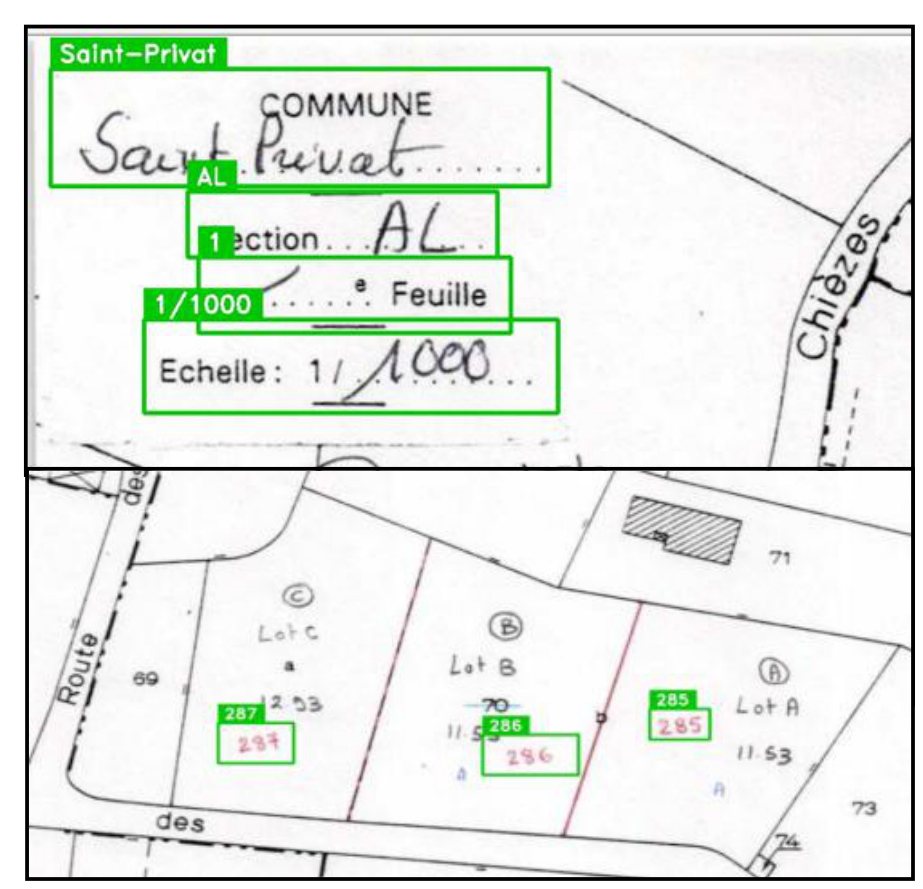
\includegraphics[width=0.6\textwidth]{img/r4p_fig2_tight.png}
  \caption{Zones de détection et affichage des boîtes englobantes sur un document d'arpentage (DMPC) par YOLOv8.}
  \label{fig:nms_exemple}
\end{figure}

Comme le montre ce résultat, YOLOv8 parvient à repérer les informations essentielles du document d'arpentage (DMPC) en traçant un cadre vert autour de chaque élément utile : le nom de la commune, la section cadastrale, le numéro de feuille et l'échelle du plan. Ces zones découpées sont ensuite transmises aux scripts de lecture pour extraire proprement le texte de chaque case.


% A RELIRE
\subsection{Prétraitement de l'image}

Envoyer un extrait d'image directement vers le moteur de lecture peut causer des erreurs si le document a été posé de travers ou si le papier est dégradé. Plusieurs traitements d'image sont appliqués avant la lecture.

Lorsqu'une feuille est numérisée avec un léger penchant, les lignes de texte ne sont plus horizontales, ce qui perturbe la lecture mot à mot. Pour corriger cela, le script applique une chaîne de traitement classique. Le filtre de Canny~\citep{canny_edge_1986} détecte d'abord les contours de l'image en mesurant les variations locales de luminosité, puis la transformée de Hough~\citep{duda_hough_1972} analyse l'espace des paramètres $(\rho, \theta)$ pour trouver les lignes les mieux représentées dans l'image :

\begin{equation}
  \rho = x \cos\theta + y \sin\theta
\end{equation}

où $\rho$ est la distance de la droite à l'origine et $\theta$ son angle par rapport à l'axe horizontal. Les lignes les plus représentées correspondent aux séparateurs de colonnes ou aux lignes de texte du document. L'angle dominant $\theta$ déduit de ces calculs définit l'inclinaison à corriger. Le script applique ensuite une rotation inverse de cet angle sur toute l'image avant de la transmettre au modèle de lecture.

Comme présenté dans l'état de l'art (section~\ref{subsec:ocr}), les archives présentent souvent du papier jauni, des taches ou de l'encre effacée. Un réglage global du contraste sur toute la page risque de faire disparaître les écritures claires sur fond clair. Le script utilise donc la méthode de binarisation par seuil local d'~\citet{otsu_threshold_1979}. L'image est découpée en fenêtres rectangulaires qui se chevauchent partiellement, et l'algorithme calcule automatiquement le seuil de séparation optimal entre l'écriture et le fond pour chaque région. Ce seuil est déterminé en maximisant la variance inter-classes :

\begin{equation}
  \sigma_B^2 = \omega_0(t)\,\omega_1(t)\,\bigl[\mu_0(t) - \mu_1(t)\bigr]^2
\end{equation}

où $\omega_0$ et $\omega_1$ sont les poids de probabilité des deux classes (fond et encre) et $\mu_0$, $\mu_1$ leurs moyennes d'intensité pour un seuil $t$ donné. Maximiser cette variance permet de séparer les deux classes de pixels, même quand leur niveau de gris varie d'une zone à l'autre du document. Cette adaptation locale fait ressortir l'écriture manuscrite et les traits légers tout en éliminant les variations de couleur dues au vieillissement du papier.

Certains documents anciens, numérisés depuis un livre ou un carnet relié, présentent une déformation en trapèze vers l'intérieur de la reliure. Dans ce cas, la simple rotation ne suffit pas à redresser les lignes de texte. Pour les détections de boîtes englobantes inclinées par YOLOv8, le script applique une transformation de perspective (homographie) qui reprend les quatre coins du cadre détecté et les projette sur un rectangle à plat via la fonction \texttt{cv2.getPerspectiveTransform} d'OpenCV :

\begin{equation}
  \begin{pmatrix} x' \\ y' \\ 1 \end{pmatrix} = H \begin{pmatrix} x \\ y \\ 1 \end{pmatrix}, \quad H \in \mathbb{R}^{3\times3}
\end{equation}

Cette correction garantit que la zone extraite est présentée au moteur de lecture sous un format plat et normalisé, quel que soit l'angle ou la déformation d'origine du document.

La Figure~\ref{fig:pretraitement_exemple} illustre le résultat de ces étapes de correction d'image.

\begin{figure}[H]
  \centering
  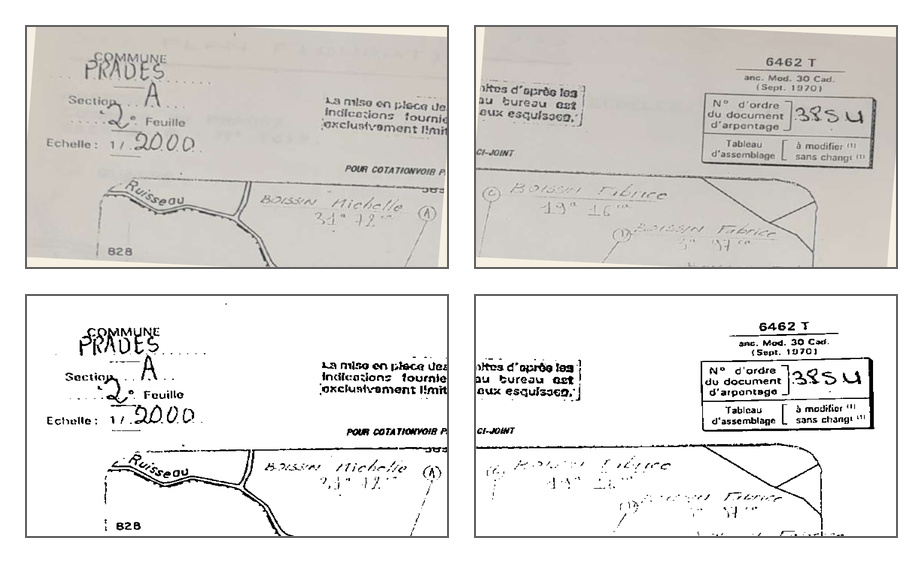
\includegraphics[width=0.85\textwidth]{img/pretraitement_vrai_plan.png}
  \caption{Zoom sur les cartouches d'un document : comparaison entre l'image numérisée inclinée à -3,5\textdegree{} (en haut) et le résultat droit après seuillage d'Otsu (en bas). L'image a volontairement été mal scannée pour les besoins de l'écrit.}
  \label{fig:pretraitement_exemple}
\end{figure}

Sur l'image brute en haut, l'inclinaison de la feuille rend la lecture des lignes difficile. Après le passage des filtres en bas, le texte est remis droit et les écritures ressortent en noir sur un fond blanc. Ce nettoyage facilite le travail du moteur de lecture.

En complément du redressement et de la binarisation, une opération de filtrage morphologique est appliquée pour éliminer les petits bruits d'encre et les bavures. Une fermeture morphologique (dilatation suivie d'une érosion par un élément structurant rectangulaire) permet de relier les traits discontinus des caractères manuscrits effacés tout en supprimant les points isolés. De plus, un rognage automatique supprime les marges noires du scanner en repérant les bords du papier, ce qui évite d'envoyer des bordures sombres inutilement aux modèles de segmentation.
% >>>>>>>>>>>>>>>>>>>




\subsection{Extraction du texte et des données clés}

Une fois les zones du document recadrées et nettoyées par le prétraitement, l'étape de lecture s'exécute via le script \texttt{outil\_ocr.py}. Cette phase contient deux approches  selon le texte du document:
\begin{itemize}
  \item Le moteur Tesseract traite les caractères tapés. Il convertit les zones imprimées en chaînes de texte.
  \item Le modèle PyLaia prend le relais pour l'écriture manuscrite. Il lit les mots lettre par lettre.
\end{itemize}

Le texte brut extrait par l'OCR contient toutefois des phrases entières, des abréviations ou du bruit entourant l'information recherchée. Pour extraire les données utiles sans écrire des dizaines de règles, l'outil s'appuie sur le modèle de reconnaissance d'entités GLiNER.

Ce dernier analyse directement la chaîne de texte brute et y recherche les champs cibles (le nom de la commune, le numéro de dossier, la section cadastrale, la date et le nom du géomètre). Pour chaque champ extrait, le modèle attribue une note de confiance comprise entre 0 et 1 :
\begin{itemize}
  \item Si le score de confiance est supérieur ou égal au seuil défini (réglé à 0,45), l'information est considérée comme fiable et pré-remplie automatiquement.
  \item Si le score de confiance est inférieur à 0,45 (dû à une tache, une écriture difficile ou une rature), l'entité est marquée comme douteuse et transférée à l'étape suivante d'arbitrage.
\end{itemize}

Ce score de confiance ne repose pas uniquement sur la probabilité calculée par le modèle GLiNER. Le script de contrôle (\texttt{coherence\_controle.py}) vient aussi vérifier la cohérence des réponses. Par exemple, si la commune trouvée existe bien dans la base de données de l'Ardèche (\texttt{ardeche.json}) et que le format de la section est correct, la note globale reste élevée. En revanche, si une lecture est étrange ou que le format ne correspond pas, le score baisse en dessous de 0,45 pour demander une confirmation par le modèle suivant.


La Figure~\ref{fig:extraction_ocr_gliner} illustre l'exécution de l'outil sur un document de type DA.

\begin{figure}[H]
  \centering
  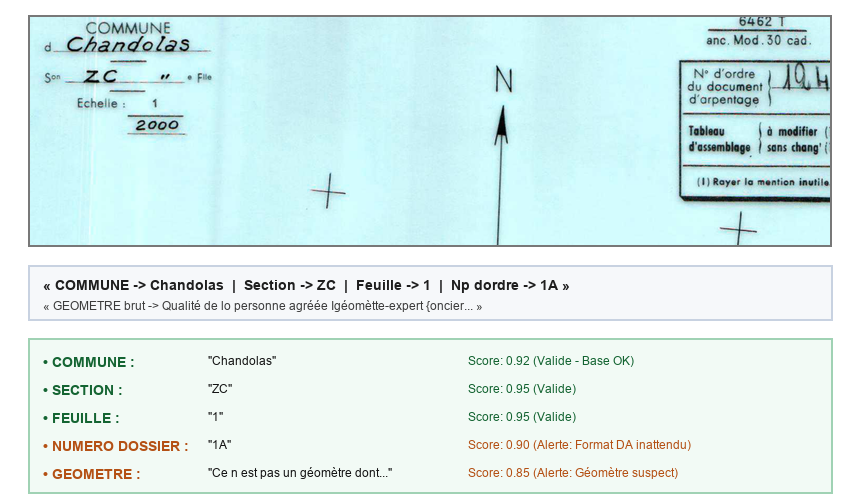
\includegraphics[width=0.9\textwidth]{img/extraction_ocr_gliner.png}
  \caption{Processus d'extraction des entités par GLiNER.} 
  \label{fig:extraction_ocr_gliner}
\end{figure}

En haut de l'image, le script découpe d'abord la zone d'intérêt du cartouche. Au milieu, le moteur de lecture extrait la chaîne de texte brute, avec ses fautes d'impression ou ses abréviations. Enfin, en bas, GLiNER et le script de vérification classent les informations dans les bons champs en leur attribuant une note de confiance et des alertes si une donnée semble fausse, l'envoyant dans ce cas à l'étape suivante d'arbitrage.

Lorsque le document contient plusieurs lignes de texte proches (par exemple dans le tableau des parcelles ou dans l'en-tête du procès-verbal), la simple extraction linéaire des mots ne suffit pas. Le script calcule le rectangle englobant de chaque mot reconnu et regroupe les termes appartenant à une même ligne selon leur chevauchement vertical. Les paires clé-valeur (comme la mention "Commune de" suivie du nom de la localité) sont associées en mesurant la distance horizontale minimale entre le libellé imprimé et la réponse manuscrite.

Pour éviter que des mots communs du vocabulaire juridique ou topographique (tels que "voie", "chemin", "parcelle", "section") ne soient interprétés à tort comme des noms de personnes ou de lieux, les réponses proposées par le modèle d'entités sont filtrées par un dictionnaire de mots exclus. Seules les entités qui passent ce filtre et qui présentent une similarité suffisante avec les référentiels régionaux sont conservées avec un score de confiance supérieur au seuil de validation.

Cette combinaison d'outils permet de traiter l'ensemble des cas d'usage sans imposer de réentraînement lourd sur chaque nouveau type de document. Comme nous l'étudierons lors de la présentation de l'interface de validation au chapitre~\ref{sec:fiabilisation}, la note de confiance attribuée à chaque champ détermine la couleur du badge affiché à l'écran, guidant ainsi l'opérateur vers les champs nécessitant une vérification prioritaire.





\subsection{Arbitrage par modèle VLM}

Le traitement par modèle VLM demande plus de temps de calcul (10 à 30 secondes par zone d'image). Il est donc réservé uniquement aux cas où la première lecture par l'OCR ou GLiNER reste incertaine (score de confiance inférieur à 0,45 ou alerte de cohérence).

Le modèle VLM \texttt{llava} tourne alors sur la machine via l'outil Ollama (port 11434). Les images ne quittent ainsi jamais l'ordinateur.

Contrairement à l'OCR qui lit le texte caractère par caractère, le modèle VLM regarde l'image de la zone dans son ensemble et répond à une consigne écrite. Par exemple, pour valider la commune, la consigne configurée dans le script est la suivante :

\begin{quote}
\textit{« Quel est le nom de la commune d'Ardèche écrit dans cette case ? Réponds uniquement par le nom de la commune, sans phrase, et répond par INCERTAIN lorsque tu n'arrive pas à une réponse plausible. »}
\end{quote}

Si le modèle parvient à lire la zone, il met à jour la valeur. S'il hésite, il répond « INCERTAIN », ce qui signale le dossier pour la vérification humaine.

La Figure~\ref{fig:ollama_vlm_schema} montre cet arbitrage sur un document issu du fonds du Géomètre B (\texttt{EXEMPLE\_}\linebreak[0]\texttt{GEOMETRE\_}\linebreak[0]\texttt{B.pdf}). L'OCR brut lit la chaîne manuscrite (\texttt{St Didier suus Aubenas}) et retient initialement la commune d'Aubenas. Le script de contrôle détecte alors une alerte de cohérence, due à une longueur anormale de caractères, ce qui déclenche automatiquement le modèle VLM. Ce dernier réexamine la zone et valide la commune exacte de Saint-Didier-sous-Aubenas.



\begin{figure}[H]
  \centering
  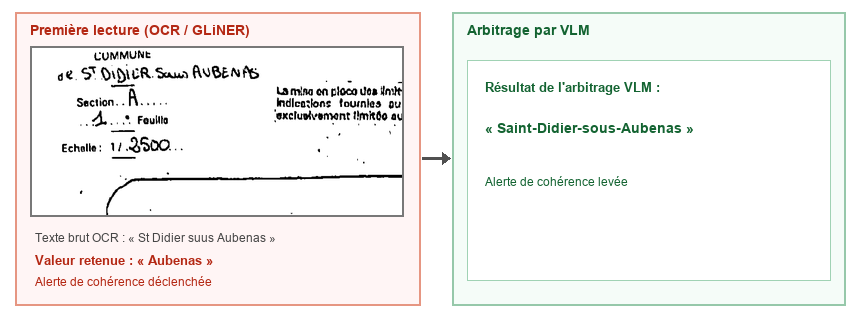
\includegraphics[width=0.95\textwidth]{img/vlm_arbitrage_exemple.png}
  \caption{Arbitrage par le modèle VLM déclenché par une alerte de cohérence sur le document du Géomètre B (\texttt{EXEMPLE\_GEOMETRE\_B.pdf}).}
  \label{fig:ollama_vlm_schema}
\end{figure}

En plus des communes, le modèle VLM est utilisé pour d'autres cas sur les documents :

\begin{itemize}
  \item Pour les choix pré-imprimés sur un DMPC, afin d'identifier l'option A, B ou C non rayée au stylo, une information qui peut être utile pour un opérateur.
  \item Pour les dates ou les jours impossibles renvoyés par la première lecture.
  \item Pour lire le texte sous les tampons ou les pliures, par exemple pour détecter le nom du géomètre-expert ayant effectué la mission.
  \item Pour les noms de propriétaires, où il est fréquemment utilisé car ils sont écrits à la main et qu'aucune règle ne permet de les identifier avec certitude.
\end{itemize}

L'utilisation de consignes textuelles ciblées permet d'adapter la sensibilité du modèle VLM selon la nature du champ. Pour réduire le temps de réponse et éviter que le modèle ne génère des phrases trop longues, la température de génération est réglée à une valeur très faible (0,1). Cette contrainte force le modèle à retourner des réponses concises et directes, immédiatement nettoyées par une fonction de filtrage qui supprime la ponctuation inutile et met en majuscules le texte extrait avant sa validation.

En cas d'échec de réponse du modèle VLM ou si le temps de calcul dépasse un seuil tolérable de 45 secondes, l'arbitrage est interrompu et la mention par défaut est attribuée au champ, pour que l'opérateur effectue lui-même la vérification dans l'interface web.

Comme indiqué lors de la présentation théorique des VLM (section~\ref{sec:vlm_execution}), cette exécution en local via l'outil Ollama garantit l'autonomie complète du cabinet sans transmettre d'images sur des serveurs externes.


\subsection{Formats de données, règles de contrôle et bilan}

Le résultat de l'extraction est enregistré sous la forme d'un fichier JSON structuré, associé à chaque document. Ce fichier regroupe l'ensemble des valeurs lues, leurs scores de confiance respectifs et les alertes générées par le contrôle de cohérence.

Pour s'assurer qu'aucune information absurde ne soit transmise à l'étape suivante, le script \texttt{coherence\_controle.py} applique une série de vérifications automatiques :

\begin{itemize}
  \item Vérification des communes : le nom extrait est comparé à la liste officielle des communes de l'Ardèche et de la Drôme (via le Code Officiel Géographique de l'INSEE). Si l'orthographe s'écarte du nom de référence, la distance de Levenshtein calcule la commune la plus proche. Si le score de correspondance est inférieur à un seuil défini (88\,\%), le champ est marqué en alerte.
  \item Cohérence temporelle : la date de l'acte doit être comprise dans une plage plausible (par exemple entre 1950 et l'année en cours). Une date située en dehors de cette plage déclenche une alerte de validation.
  \item Format des références : les numéros de dossiers et les références cadastrales sont contrôlés par des expressions régulières (regex) pour vérifier leur structure (par exemple, une section cadastrale composée de 1 ou 2 lettres, suivie d'un numéro de parcelle entier).
\end{itemize}

Ce schéma de données structuré permet de conserver la traçabilité complète de chaque extrait. Comme nous le verrons lors de la phase d'exportation vers Géofoncier (chapitre~\ref{sec:integration}), ce fichier JSON sert de socle pour construire la requête REST transmise à l'API.


À la fin de ce processus, toutes les informations contrôlées sont enregistrées dans un fichier JSON propre pour chaque document.

Même si le système automatise la majorité du travail de lecture, des erreurs peuvent persister : une information est parfois illisible, sujette à interprétation, ou simplement hors de portée des modèles. Un contrôle humain est alors nécessaire. Le chapitre suivant présente la partie fiabilisation et l'interface graphique permettant à l'utilisateur de contrôler et valider les dossiers avant l'envoi final sur Géofoncier.


\subsection{Constitution du jeu de données d'entraînement}

Le modèle YOLOv8 utilisé pour découper les zones d'intérêt sur les pages de documents doit être entraîné sur des exemples issus du fonds du cabinet. Un modèle pré-entraîné sur des images génériques est incapable de localiser correctement des zones aussi spécifiques que le cartouche d'un DMPC ou le tableau de parcelles d'un DA.

Pour constituer ce jeu d'entraînement, 500 pages ont été sélectionnées parmi les fonds des deux géomètres. La sélection couvre plusieurs générations de formulaires (avant et après 1980), plusieurs niveaux de qualité de numérisation (200 à 300 DPI), plusieurs types d'actes (DMPC, DA, PV de bornage) et plusieurs états de conservation (papier propre, papier jauni, tampon en marge, rature). Cette diversité est indispensable pour que le modèle apprenne à détecter les zones dans des conditions variables et ne soit pas limité aux seuls documents en parfait état.

Les 500 pages ont été annotées manuellement à l'aide du logiciel libre Label Studio, installé en local sur la machine du cabinet. Label Studio permet de tracer des boîtes englobantes sur des images et d'associer une étiquette à chaque zone. Les classes définies pour ce projet sont les suivantes : \texttt{commune}, \texttt{section}, \texttt{parcelles}, \texttt{date}, \texttt{geometre} et \texttt{tampon}.



Chaque page a été annotée par une seule personne et vérifiée par une seconde lors d'une phase de relecture. Les boîtes ont été tracées au plus près du contenu, sans inclure les marges extérieures du formulaire. Au total, environ 3\,200 boîtes englobantes ont été produites sur les 500 pages, soit une moyenne de 6,4 zones annotées par page.

Les 500 images annotées ont été réparties en trois sous-ensembles : 70\,\% pour l'entraînement (350 images), 15\,\% pour la validation (75 images) et 15\,\% pour le test final (75 images). L'entraînement a été réalisé sur 50 époques avec le modèle léger \texttt{yolov8n.pt}, ce qui prend environ 40 minutes sur la carte graphique NVIDIA du poste de travail. Le score de détection moyen atteint sur le jeu de test est de mAP50 = 0,94, ce qui signifie que le modèle localise correctement 94\,\% des zones avec un seuil de chevauchement de 50\,\%.

Le système est conçu pour être ré-entraînable sans intervention technique complexe. Chaque fois qu'un lot de nouveaux documents est annoté, le script de ré-entraînement peut être relancé depuis un fichier de commandes qui exporte les annotations et démarre l'entraînement. Le modèle mis à jour remplace automatiquement l'ancien sans modifier le reste du code.


\subsection{Gestion des exceptions et stratégies de repli}

Dans une chaîne de traitement automatisée traitant des documents numérisés aux formats variés, des erreurs de calcul ou des échecs de détection peuvent survenir à chaque étape. Pour éviter qu'un fichier défectueux ne bloque l'ensemble du traitement par lot, le script principal intègre une gestion des exceptions associant des stratégies de repli.

Si le modèle YOLOv8 ne retourne aucune boîte englobante sur une page (par exemple en cas de document au format non standard ou très sombre), le script bascule automatiquement sur un découpage géométrique par défaut. Les coordonnées des zones sont calculées à partir de ratios fixes (cartouche supérieur droit entre 0\,\% et 25\,\% de la hauteur, tableau central entre 25\,\% et 75\,\% de la hauteur). Un avertissement est inscrit dans le fichier JSON pour signaler le recours au découpage par défaut.

Si la carte graphique est sollicitée par une autre application ou si la mémoire vidéo est insuffisante lors du chargement des modèles PyLaia ou GLiNER, le système bascule automatiquement l'exécution du modèle concerné sur le processeur central (CPU). Le temps de calcul s'allonge, mais le traitement continue sans interruption.

Lorsque l'OCR extrait des chaînes de caractères contenant des octets invalides ou des symboles non imprimables (fréquent sur les tampons baveux), la fonction de nettoyage filtre les caractères hors de la plage UTF-8 standard. Si la chaîne nettoyée est vide, le champ prend la valeur \texttt{INCERTAIN} et le score de confiance est mis à 0, ce qui signale le dossier pour la relecture dans l'interface Streamlit (chapitre~\ref{sec:fiabilisation}).

Le Tableau~\ref{tab:strategies_repli} récapitule les principales exceptions gérées par l'architecture et les réponses apportées.

\begin{table}[H]
  \centering
  \caption{Synthèse des exceptions gérées par la chaîne de traitement et mécanismes de repli.}
  \label{tab:strategies_repli}
  \small
  \begin{tabular}{p{4.5cm} p{4.5cm} p{5.5cm}}
    \toprule
    \textbf{Événement déclencheur} & \textbf{Détection / Exception} & \textbf{Stratégie de repli appliquée} \\
    \midrule
    Aucune boîte YOLO trouvée & Liste de boîtes vide & Découpage géométrique par ratios de page. \\
    Mémoire GPU insuffisante & Exception mémoire CUDA & Bascule automatique de l'inférence sur CPU. \\
    Texte OCR illisible ou vide & Chaîne vide après nettoyage & Champ marqué \texttt{INCERTAIN}, alerte dans l'IHM. \\
    Fichier PDF corrompu & Erreur de lecture fichier & Document déplacé dans \texttt{errors/}, log d'échec. \\
    API Géofoncier indisponible & Erreur de connexion réseau & Stockage du dictionnaire dans \texttt{pending\_api/}. \\
    \bottomrule
  \end{tabular}
\end{table}

Cette organisation garantit la robustesse de l'application sur de grands volumes de fichiers. Un document comportant une anomalie est isolé sans interrompre le traitement des autres pièces du lot.

De plus, l'ensemble des événements et erreurs survenus lors de l'exécution est consigné dans un fichier de journalisation quotidien (\texttt{traitement.log}). Ce journal d'erreurs indique l'horodatage précis, le nom du fichier concerné, le module informatique à l'origine de l'alerte ainsi que le code de l'erreur. Cette traçabilité permet au responsable informatique du cabinet d'identifier rapidement les documents problématiques et d'ajuster les règles de repli si nécessaire.
% >>>>>>>>>>>>>>>>>>>








